% Options for packages loaded elsewhere
\PassOptionsToPackage{unicode}{hyperref}
\PassOptionsToPackage{hyphens}{url}
%
\documentclass[
]{article}
\title{Cronchbach's alpha and FAs on scales}
\author{}
\date{\vspace{-2.5em}}

\usepackage{amsmath,amssymb}
\usepackage{lmodern}
\usepackage{iftex}
\ifPDFTeX
  \usepackage[T1]{fontenc}
  \usepackage[utf8]{inputenc}
  \usepackage{textcomp} % provide euro and other symbols
\else % if luatex or xetex
  \usepackage{unicode-math}
  \defaultfontfeatures{Scale=MatchLowercase}
  \defaultfontfeatures[\rmfamily]{Ligatures=TeX,Scale=1}
\fi
% Use upquote if available, for straight quotes in verbatim environments
\IfFileExists{upquote.sty}{\usepackage{upquote}}{}
\IfFileExists{microtype.sty}{% use microtype if available
  \usepackage[]{microtype}
  \UseMicrotypeSet[protrusion]{basicmath} % disable protrusion for tt fonts
}{}
\makeatletter
\@ifundefined{KOMAClassName}{% if non-KOMA class
  \IfFileExists{parskip.sty}{%
    \usepackage{parskip}
  }{% else
    \setlength{\parindent}{0pt}
    \setlength{\parskip}{6pt plus 2pt minus 1pt}}
}{% if KOMA class
  \KOMAoptions{parskip=half}}
\makeatother
\usepackage{xcolor}
\IfFileExists{xurl.sty}{\usepackage{xurl}}{} % add URL line breaks if available
\IfFileExists{bookmark.sty}{\usepackage{bookmark}}{\usepackage{hyperref}}
\hypersetup{
  pdftitle={Cronchbach's alpha and FAs on scales},
  hidelinks,
  pdfcreator={LaTeX via pandoc}}
\urlstyle{same} % disable monospaced font for URLs
\usepackage[margin=1in]{geometry}
\usepackage{graphicx}
\makeatletter
\def\maxwidth{\ifdim\Gin@nat@width>\linewidth\linewidth\else\Gin@nat@width\fi}
\def\maxheight{\ifdim\Gin@nat@height>\textheight\textheight\else\Gin@nat@height\fi}
\makeatother
% Scale images if necessary, so that they will not overflow the page
% margins by default, and it is still possible to overwrite the defaults
% using explicit options in \includegraphics[width, height, ...]{}
\setkeys{Gin}{width=\maxwidth,height=\maxheight,keepaspectratio}
% Set default figure placement to htbp
\makeatletter
\def\fps@figure{htbp}
\makeatother
\setlength{\emergencystretch}{3em} % prevent overfull lines
\providecommand{\tightlist}{%
  \setlength{\itemsep}{0pt}\setlength{\parskip}{0pt}}
\setcounter{secnumdepth}{-\maxdimen} % remove section numbering
\ifLuaTeX
  \usepackage{selnolig}  % disable illegal ligatures
\fi

\begin{document}
\maketitle

{
\setcounter{tocdepth}{2}
\tableofcontents
}
\newpage

\hypertarget{kahan-et-al-2007-scale}{%
\section{Kahan et al (2007) scale}\label{kahan-et-al-2007-scale}}

\hypertarget{cronbachs-alpha-test-on-the-kahan-et-al-2007-scale}{%
\subsection{Cronbach's alpha test on the Kahan et al (2007)
scale}\label{cronbachs-alpha-test-on-the-kahan-et-al-2007-scale}}

\textbf{Kahan et al (2007) scale}

Individualism - Communitarinism

\begin{itemize}
\tightlist
\item
  \textbf{K\_IINTRFER} The government interferes far too much in our
  everyday lives.
\item
  \textbf{K\_IPRIVACY} The government should stop telling people how to
  live their lives.
\item
  \textbf{K\_IPROTECT} It's not the government's business to try to
  protect people from themselves.
\item
  \textbf{K\_SHARM} Sometimes the government needs to make laws that
  keep people from hurting themselves.
\item
  \textbf{K\_SLIMCHOI} The government should put limits on the choices
  individuals can make so they don't get in the way of what's good for
  society.
\item
  \textbf{K\_SPROTECT} The government should do more to advance
  society's goals, even if that means limiting the freedom and choices
  of individuals.
\end{itemize}

Hierarchy -Egalitarianism

\begin{itemize}
\tightlist
\item
  \textbf{K\_HEQUAL} We have gone too far in pushing equal rights in
  this country.
\item
  \textbf{K\_HREVDIS1} Nowadays it seems like there is just as much
  discrimination against upper castes as there is against Dalits.
\item
  \textbf{K\_EDISCRIM} Discrimination against minorities is still a very
  serious problem in our society.
\item
  \textbf{K\_ERADEQ1} We need to dramatically reduce inequalities
  between the rich and the poor.
\item
  \textbf{K\_EWEALTH} Our society would be better off if the
  distribution of wealth was more equal.
\item
  \textbf{K\_ERADEQ2} We need to dramatically reduce inequalities
  between men and women.
\end{itemize}

KahanI weak alpha = 0.29, KahanS strong alpha = 0.71 Hierarchy
-Egalitarianism strong alpha = 0.71 reasons for this could be that the
individualism items are not well adapted to the Indian population final
items alpha = 0.75

\newpage

\hypertarget{cfa-on-the-kahan-scale}{%
\section{CFA on the Kahan scale}\label{cfa-on-the-kahan-scale}}

Since this a well used scale with theoretical basis for factor
distinctions and there are also previous studies that used the same
scale I did CFA not exploratory FA.

\begin{verbatim}
## lavaan 0.6.15 ended normally after 16 iterations
## 
##   Estimator                                         ML
##   Optimization method                           NLMINB
##   Number of model parameters                        13
## 
##   Number of observations                           749
## 
## Model Test User Model:
##                                                       
##   Test statistic                                42.022
##   Degrees of freedom                                 8
##   P-value (Chi-square)                           0.000
## 
## Model Test Baseline Model:
## 
##   Test statistic                              1057.597
##   Degrees of freedom                                15
##   P-value                                        0.000
## 
## User Model versus Baseline Model:
## 
##   Comparative Fit Index (CFI)                    0.967
##   Tucker-Lewis Index (TLI)                       0.939
## 
## Loglikelihood and Information Criteria:
## 
##   Loglikelihood user model (H0)              -6375.464
##   Loglikelihood unrestricted model (H1)      -6354.452
##                                                       
##   Akaike (AIC)                               12776.927
##   Bayesian (BIC)                             12836.971
##   Sample-size adjusted Bayesian (SABIC)      12795.691
## 
## Root Mean Square Error of Approximation:
## 
##   RMSEA                                          0.075
##   90 Percent confidence interval - lower         0.054
##   90 Percent confidence interval - upper         0.099
##   P-value H_0: RMSEA <= 0.050                    0.027
##   P-value H_0: RMSEA >= 0.080                    0.396
## 
## Standardized Root Mean Square Residual:
## 
##   SRMR                                           0.042
## 
## Parameter Estimates:
## 
##   Standard errors                             Standard
##   Information                                 Expected
##   Information saturated (h1) model          Structured
## 
## Latent Variables:
##                    Estimate  Std.Err  z-value  P(>|z|)   Std.lv  Std.all
##   KahanS =~                                                             
##     K_SHARM           0.726    0.044   16.405    0.000    0.726    0.639
##     K_SLIMCHOI        0.938    0.047   20.057    0.000    0.938    0.787
##     K_SPROTECT        0.714    0.046   15.605    0.000    0.714    0.608
##   KahanH =~                                                             
##     K_ERADEQ1         0.750    0.039   19.198    0.000    0.750    0.748
##     K_EWEALTH         0.642    0.045   14.323    0.000    0.642    0.560
##     K_ERADEQ2         0.782    0.042   18.656    0.000    0.782    0.726
## 
## Covariances:
##                    Estimate  Std.Err  z-value  P(>|z|)   Std.lv  Std.all
##   KahanS ~~                                                             
##     KahanH            0.528    0.040   13.121    0.000    0.528    0.528
## 
## Variances:
##                    Estimate  Std.Err  z-value  P(>|z|)   Std.lv  Std.all
##    .K_SHARM           0.764    0.053   14.457    0.000    0.764    0.592
##    .K_SLIMCHOI        0.542    0.062    8.700    0.000    0.542    0.381
##    .K_SPROTECT        0.868    0.057   15.293    0.000    0.868    0.630
##    .K_ERADEQ1         0.441    0.042   10.466    0.000    0.441    0.440
##    .K_EWEALTH         0.903    0.055   16.369    0.000    0.903    0.687
##    .K_ERADEQ2         0.548    0.048   11.399    0.000    0.548    0.473
##     KahanS            1.000                               1.000    1.000
##     KahanH            1.000                               1.000    1.000
\end{verbatim}

\newpage

\hypertarget{eco-pol-value-scale}{%
\section{Eco-pol value scale}\label{eco-pol-value-scale}}

\textbf{Scale 1 : The economic -political values of the perceiver}

\begin{itemize}
\tightlist
\item
  \textbf{DECISIONDECEN} Local politicians shouldn't have to ask
  permission from the central government to implement policies
\item
  \textbf{DECISIONCEN} Laws and policies would be implemented more
  smoothly if more power lay with the central government.
\item
  \textbf{SYSTEMTOTAL} It is good to have a strong leader who does not
  have to bother with elections.
\item
  \textbf{SYSTEMTECHNO} Experts, not the government, should make
  decisions according to what they think is best for the country.
\item
  \textbf{SYSTEMDEMO} It is very important to have a democratic
  political system because it ensures that no individual leader has too
  much power.
\item
  \textbf{SYSTEMRELIGION} There should be a system governed by religious
  law.
\item
  \textbf{INDUSTRYSMALL} Large corporations are destroying the local
  industries in India and benefiting only a handful of people.
\item
  \textbf{INDUSTRYLARGE} Large scale industries are required for the
  development of the country that will benefit everyone
\item
  \textbf{ECONOMYLOCAL} India would be better off if foreign companies
  didn't come to here
\item
  \textbf{ECONOMYGLOBAL} Foreign companies have led to a range of
  benefits for the Indian people and society
\item
  \textbf{DEVOVERENV} Economic growth and creating jobs should be
  prioritized over environmental protection
\item
  \textbf{ENVOVERDEV} Polluting industries that spoil the environment
  should be shut down even if it costs people their jobs
\item
  \textbf{OWNERPVT} All businesses and industries should be owned
  privately
\item
  \textbf{OWNERPUB} The government should own most large businesses and
  industries
\item
  \textbf{OWNERREG} Regardless of ownership, the government should pass
  strong regulations and implement them
\item
  \textbf{OWNERNOREG} There is too much red-tape and the government
  should not interfere with businesses and industries
\item
  \textbf{WEALTHLIM} A limit should be put to how much wealth a person
  can amass
\item
  \textbf{MECHANISATION} Rapid mechanization of work is taking away jobs
  from workers in this country
\end{itemize}

\hypertarget{cronbachs-alpha-test-on-scale-1-economic--political-values-of-the-perceiver}{%
\subsection{Cronbach's Alpha Test on Scale 1: Economic -Political Values
of the
Perceiver}\label{cronbachs-alpha-test-on-scale-1-economic--political-values-of-the-perceiver}}

\begin{verbatim}
## 
## Reliability analysis   
##  raw_alpha std.alpha G6(smc) average_r S/N   ase mean   sd median_r
##       0.75      0.76    0.79      0.15 3.2 0.014  3.5 0.56     0.16
\end{verbatim}

\newpage

\textbf{Scale 2 : Economic and Political characteristics of the energy
technology scale - Nuclear energy}

\begin{itemize}
\tightlist
\item
  \textbf{DISPLACENUCLER} Nuclear energy is leading to displacement of
  people from their land
\item
  \textbf{POLLUTENUCLEAR} Nuclear energy increases pollution of
  air/water/land
\item
  \textbf{HEALTHNUCLEAR} Nuclear energy poses a great risk to the health
  of people living around it
\item
  \textbf{JOBSNUCLEAR} Nuclear energy will bring jobs to the local
  community
\item
  \textbf{BEAUTYNUCLEAR} Nuclear energy spoils the natural beauty of the
  landscape
\item
  \textbf{PRIDENUCLEAR} I would be proud if my community used nuclear
  energy
\item
  \textbf{NPRIDENUCLEAR} Nuclear energy is a mark of pride for our
  nation
\item
  \textbf{DEVNUCLEAR} Nuclear energy pushes forward the country's
  development
\item
  \textbf{PROSPERNUCLEAR} Nuclear energy brings economic prosperity to
  the surrounding regions
\item
  \textbf{RELYNUCLEAR} I don't like the idea that I have to rely on the
  government for electricity from nuclear energy
\end{itemize}

\hypertarget{cronbachs-alpha-test-on-scale-2-eco-pol-characteristics-of-the-technology---nuclear-energy}{%
\subsection{Cronbach's alpha test on Scale 2 : Eco-Pol Characteristics
of the Technology - Nuclear
Energy}\label{cronbachs-alpha-test-on-scale-2-eco-pol-characteristics-of-the-technology---nuclear-energy}}

\begin{verbatim}
## 
## Reliability analysis   
##  raw_alpha std.alpha G6(smc) average_r S/N   ase mean   sd median_r
##       0.68      0.69    0.76      0.18 2.2 0.021  3.4 0.61     0.19
\end{verbatim}

\hypertarget{cronbachs-alpha-test-on-the-combined-scale.}{%
\subsection{Cronbach's Alpha Test on the Combined
Scale.}\label{cronbachs-alpha-test-on-the-combined-scale.}}

\begin{verbatim}
## 
## Reliability analysis   
##  raw_alpha std.alpha G6(smc) average_r S/N   ase mean   sd median_r
##        0.8       0.8    0.84      0.14   4 0.014  3.3 0.49     0.13
\end{verbatim}

\newpage

\hypertarget{fa-on-all-ecopol-variables-except-systems-of-governance}{%
\section{FA on All Ecopol Variables (except systems of
governance)}\label{fa-on-all-ecopol-variables-except-systems-of-governance}}

\hypertarget{two-factor-solution-mr1-people-centered-development-and-mr2-nationalist-development}{%
\subsection{Two factor solution : MR1 people centered development and
MR2 nationalist
development}\label{two-factor-solution-mr1-people-centered-development-and-mr2-nationalist-development}}

\textbf{MR1 People Centered Development: Pdevelop}

HEALTHNUCLEAR - Nuclear energy poses a great risk to the health of
people living around it.

BEAUTYNUCLEAR - Nuclear energy spoils the natural beauty of the
landscape.

MECHANISATION - Rapid mechanization of work is taking away jobs from
workers in this country.

INDUSTRYSMALL - Large corporations are destroying the local industries
in India and benefiting only a handful of people.

DISPLACENUCLEAR- Nuclear energy is leading to displacement of people
from their land.

POLLUTENUCLEAR- Nuclear energy increases pollution of air/water/land.

OWNERREG- Regardless of ownership, the government should pass strong
regulations and implement them.

\textbf{MR2 Nationalist Development: Ndevelop}

DEVNUCLEAR - Nuclear energy pushes forward the country's development.

PRIDENUCLEAR- I would be proud if my community used nuclear energy.

NPRIDENUCLEAR- Nuclear energy is a mark of pride for our nation.

PROSPERNUCLEAR-Nuclear energy brings economic prosperity to the
surrounding regions.

INDUSTRYLARGE- Large scale industries are required for the development
of the country that will benefit everyone.

\begin{verbatim}
## Factor Analysis using method =  minres
## Call: fa(r = ecopolall, nfactors = 2, rotate = "varimax")
## Standardized loadings (pattern matrix) based upon correlation matrix
##                 item   MR1   MR2     h2   u2 com
## HEALTHNUCLEAR     17  0.67       0.4460 0.55 1.0
## BEAUTYNUCLEAR     19  0.62       0.3869 0.61 1.0
## DISPLACENUCLEAR   15  0.58       0.3718 0.63 1.2
## POLLUTENUCLEAR    16  0.58       0.3355 0.66 1.0
## OWNERREG          14  0.56       0.3245 0.68 1.1
## MECHANISATION      2  0.54       0.3318 0.67 1.3
## INDUSTRYSMALL      6  0.52       0.2743 0.73 1.0
## ENVOVERDEV         9             0.1554 0.84 1.1
## OWNERPUB          13             0.1555 0.84 1.2
## SYSTEMDEMO        25             0.2159 0.78 2.0
## DECISIONDECEN      3             0.1008 0.90 1.0
## WEALTHLIM          1             0.1576 0.84 2.0
## ECONOMYLOCAL       8             0.0100 0.99 1.9
## DEVNUCLEAR        22        0.64 0.4424 0.56 1.1
## PRIDENUCLEAR      20        0.63 0.4551 0.54 1.3
## NPRIDENUCLEAR     21        0.58 0.3684 0.63 1.2
## PROSPERNUCLEAR    23        0.56 0.3300 0.67 1.1
## RELYNUCLEAR       24             0.1855 0.81 1.0
## JOBSNUCLEAR       18             0.2223 0.78 1.5
## INDUSTRYLARGE      5             0.1904 0.81 1.6
## ECONOMYGLOBAL      7             0.2117 0.79 2.0
## OWNERNOREG        12             0.1015 0.90 1.4
## DECISIONCEN        4             0.0996 0.90 1.7
## OWNERPVT          11             0.0407 0.96 1.9
## DEVOVERENV        10             0.0087 0.99 1.0
## 
##                        MR1  MR2
## SS loadings           3.37 2.55
## Proportion Var        0.13 0.10
## Cumulative Var        0.13 0.24
## Proportion Explained  0.57 0.43
## Cumulative Proportion 0.57 1.00
## 
## Mean item complexity =  1.3
## Test of the hypothesis that 2 factors are sufficient.
## 
## The degrees of freedom for the null model are  300  and the objective function was  6.13 with Chi Square of  2636.59
## The degrees of freedom for the model are 251  and the objective function was  2.28 
## 
## The root mean square of the residuals (RMSR) is  0.07 
## The df corrected root mean square of the residuals is  0.08 
## 
## The harmonic number of observations is  440 with the empirical chi square  1347.65  with prob <  2.4e-149 
## The total number of observations was  440  with Likelihood Chi Square =  978.9  with prob <  1.6e-86 
## 
## Tucker Lewis Index of factoring reliability =  0.626
## RMSEA index =  0.081  and the 90 % confidence intervals are  0.076 0.087
## BIC =  -548.88
## Fit based upon off diagonal values = 0.85
## Measures of factor score adequacy             
##                                                    MR1  MR2
## Correlation of (regression) scores with factors   0.91 0.88
## Multiple R square of scores with factors          0.83 0.78
## Minimum correlation of possible factor scores     0.65 0.57
\end{verbatim}

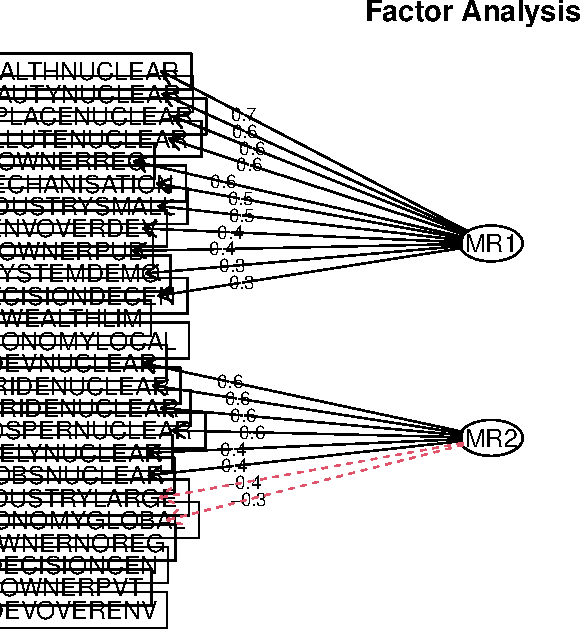
\includegraphics{module2PCAs_files/figure-latex/unnamed-chunk-8-1.pdf}

\newpage

\hypertarget{fa-on-scale-1---only-eco-pol-values-of-the-perceiver-scale.}{%
\section{FA on Scale 1 - only eco-pol values of the perceiver
scale.}\label{fa-on-scale-1---only-eco-pol-values-of-the-perceiver-scale.}}

Four Factor Solution -

\textbf{MR1 Problems of industrialisation}

MECHANISATION- Rapid mechanization of work is taking away jobs from
workers in this country

OWNERREG- Regardless of ownership, the government should pass strong
regulations and implement them.

WEALTHLIM- A limit should be put to how much wealth a person can amass

\textbf{MR3 Local Economy And Decision Making}

INDUSTRYSMALL- Large corporations are destroying the local industries in
India and benefiting only a handful of people

ECONOMYLOCAL- India would be better off if foreign companies didn't come
to here

DECISIONDECEN- Local politicians shouldn't have to ask permission from
the central government to implement policies

\textbf{MR4 Centralised and Large Industry}

DECISIONCEN- Laws and policies would be implemented more smoothly if
more power lay with the central government

ECONOMYGLOBAL- Foreign companies have led to a range of benefits for the
Indian people and society

OWNERNOREG- There is too much red-tape and the government should not
interfere with businesses and industries

INDUSTRYLARGE- Large scale industries are required for the development
of the country that will benefit everyone

\textbf{MR2 Development and Business Ownership}

DEVOVERENV- Economic growth and creating jobs should be prioritized over
environmental protection

OWNERPVT- All businesses and industries should be owned privately

OWNERPUB- The government should own most large businesses and industries

ENVOVERDEV- Polluting industries that spoil the environment should be
shut down even if it costs people their jobs

\begin{verbatim}
## 
## Reliability analysis   
## Call: alpha(x = ecopolval, check.keys = TRUE)
## 
##   raw_alpha std.alpha G6(smc) average_r S/N   ase mean   sd median_r
##       0.71      0.72    0.74      0.15 2.5 0.016  3.5 0.58     0.16
## 
##     95% confidence boundaries 
##          lower alpha upper
## Feldt     0.68  0.71  0.74
## Duhachek  0.68  0.71  0.74
## 
##  Reliability if an item is dropped:
##                raw_alpha std.alpha G6(smc) average_r S/N alpha se var.r med.r
## WEALTHLIM           0.69      0.69    0.72      0.15 2.2    0.017 0.014  0.15
## MECHANISATION       0.69      0.69    0.72      0.15 2.3    0.017 0.014  0.15
## INDUSTRYSMALL       0.68      0.69    0.71      0.15 2.2    0.017 0.014  0.15
## ECONOMYGLOBAL-      0.69      0.70    0.72      0.15 2.3    0.017 0.014  0.15
## ENVOVERDEV          0.68      0.69    0.71      0.14 2.2    0.018 0.014  0.15
## OWNERNOREG-         0.70      0.71    0.73      0.16 2.4    0.016 0.013  0.17
## OWNERPUB            0.67      0.68    0.70      0.14 2.1    0.018 0.013  0.14
## OWNERREG            0.68      0.69    0.71      0.15 2.2    0.017 0.014  0.15
## DECISIONDECEN       0.70      0.71    0.73      0.16 2.4    0.016 0.015  0.17
## DECISIONCEN-        0.70      0.71    0.73      0.16 2.4    0.016 0.014  0.17
## INDUSTRYLARGE-      0.70      0.70    0.72      0.15 2.3    0.017 0.014  0.16
## ECONOMYLOCAL        0.70      0.71    0.73      0.16 2.4    0.016 0.014  0.17
## DEVOVERENV-         0.72      0.72    0.74      0.17 2.6    0.015 0.012  0.17
## OWNERPVT            0.72      0.73    0.75      0.17 2.7    0.015 0.011  0.18
## 
##  Item statistics 
##                  n raw.r std.r r.cor r.drop mean  sd
## WEALTHLIM      721  0.53  0.53  0.49  0.401  3.7 1.3
## MECHANISATION  721  0.50  0.52  0.47  0.386  4.0 1.1
## INDUSTRYSMALL  721  0.54  0.54  0.50  0.408  3.5 1.3
## ECONOMYGLOBAL- 721  0.48  0.49  0.42  0.349  3.5 1.2
## ENVOVERDEV     721  0.58  0.57  0.54  0.461  3.6 1.3
## OWNERNOREG-    721  0.40  0.40  0.33  0.259  3.2 1.2
## OWNERPUB       721  0.62  0.62  0.60  0.509  3.4 1.2
## OWNERREG       721  0.54  0.55  0.50  0.423  3.6 1.2
## DECISIONDECEN  721  0.43  0.42  0.33  0.282  3.0 1.3
## DECISIONCEN-   721  0.41  0.42  0.34  0.272  3.6 1.2
## INDUSTRYLARGE- 721  0.45  0.47  0.40  0.328  3.9 1.2
## ECONOMYLOCAL   721  0.41  0.41  0.33  0.272  3.3 1.3
## DEVOVERENV-    721  0.32  0.29  0.19  0.148  3.4 1.4
## OWNERPVT       721  0.25  0.23  0.12  0.092  3.2 1.3
## 
## Non missing response frequency for each item
##                  1    2    3    4    5 miss
## WEALTHLIM     0.07 0.15 0.15 0.30 0.33    0
## MECHANISATION 0.03 0.13 0.12 0.28 0.44    0
## INDUSTRYSMALL 0.06 0.24 0.19 0.18 0.33    0
## ECONOMYGLOBAL 0.21 0.39 0.16 0.17 0.07    0
## ENVOVERDEV    0.08 0.17 0.13 0.32 0.30    0
## OWNERNOREG    0.19 0.23 0.29 0.20 0.09    0
## OWNERPUB      0.07 0.19 0.18 0.31 0.24    0
## OWNERREG      0.03 0.17 0.22 0.28 0.29    0
## DECISIONDECEN 0.14 0.29 0.21 0.16 0.20    0
## DECISIONCEN   0.24 0.38 0.17 0.13 0.07    0
## INDUSTRYLARGE 0.37 0.36 0.11 0.10 0.05    0
## ECONOMYLOCAL  0.08 0.22 0.22 0.23 0.24    0
## DEVOVERENV    0.31 0.27 0.13 0.16 0.14    0
## OWNERPVT      0.12 0.22 0.24 0.21 0.21    0
\end{verbatim}

\begin{verbatim}
## Factor Analysis using method =  minres
## Call: fa(r = ecopolval, nfactors = 4, rotate = "varimax")
## Standardized loadings (pattern matrix) based upon correlation matrix
##               item   MR1   MR3   MR4   MR2   h2   u2 com
## OWNERREG         8  0.54                   0.37 0.63 1.5
## MECHANISATION    2  0.51                   0.33 0.67 1.6
## WEALTHLIM        1  0.48                   0.30 0.70 1.6
## INDUSTRYSMALL    3        0.53             0.41 0.59 1.8
## ECONOMYLOCAL    12        0.52             0.29 0.71 1.1
## DECISIONDECEN    9                         0.13 0.87 2.0
## DECISIONCEN     10              0.49       0.28 0.72 1.4
## ECONOMYGLOBAL    4              0.48       0.30 0.70 1.6
## OWNERNOREG       6              0.47       0.40 0.60 2.2
## INDUSTRYLARGE   11              0.43       0.30 0.70 1.9
## DEVOVERENV      13                   -0.54 0.29 0.71 1.0
## OWNERPVT        14                    0.51 0.27 0.73 1.1
## ENVOVERDEV       5                    0.46 0.43 0.57 2.5
## OWNERPUB         7                    0.43 0.43 0.57 3.2
## 
##                        MR1  MR3  MR4  MR2
## SS loadings           1.21 1.19 1.09 1.04
## Proportion Var        0.09 0.09 0.08 0.07
## Cumulative Var        0.09 0.17 0.25 0.32
## Proportion Explained  0.27 0.26 0.24 0.23
## Cumulative Proportion 0.27 0.53 0.77 1.00
## 
## Mean item complexity =  1.8
## Test of the hypothesis that 4 factors are sufficient.
## 
## The degrees of freedom for the null model are  91  and the objective function was  2.17 with Chi Square of  1549.03
## The degrees of freedom for the model are 41  and the objective function was  0.23 
## 
## The root mean square of the residuals (RMSR) is  0.03 
## The df corrected root mean square of the residuals is  0.05 
## 
## The harmonic number of observations is  721 with the empirical chi square  147.5  with prob <  6.2e-14 
## The total number of observations was  721  with Likelihood Chi Square =  163.15  with prob <  1.7e-16 
## 
## Tucker Lewis Index of factoring reliability =  0.813
## RMSEA index =  0.064  and the 90 % confidence intervals are  0.054 0.075
## BIC =  -106.66
## Fit based upon off diagonal values = 0.97
## Measures of factor score adequacy             
##                                                    MR1  MR3  MR4  MR2
## Correlation of (regression) scores with factors   0.74 0.76 0.73 0.77
## Multiple R square of scores with factors          0.54 0.57 0.54 0.59
## Minimum correlation of possible factor scores     0.08 0.14 0.08 0.19
\end{verbatim}

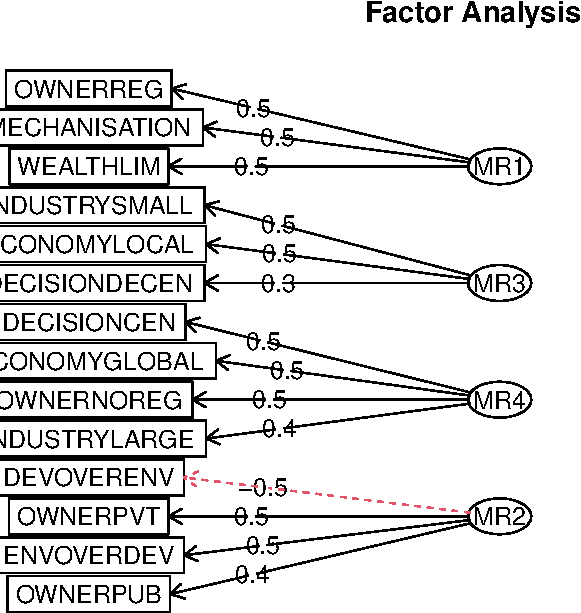
\includegraphics{module2PCAs_files/figure-latex/unnamed-chunk-9-1.pdf}

\newpage

\hypertarget{factor-analysis-on-scale-2---eco-pol-characteristics-of-the-technology---nuclear-energy}{%
\section{Factor analysis on Scale 2 - Eco-Pol characteristics of the
technology - Nuclear
Energy}\label{factor-analysis-on-scale-2---eco-pol-characteristics-of-the-technology---nuclear-energy}}

Two Factor Solution - positive versus negative characteristics

\textbf{MR1 Negative Characteristics}

HEALTHNUCLEAR - Nuclear energy poses a great risk to the health of
people living around it.

BEAUTYNUCLEAR - Nuclear energy spoils the natural beauty of the
landscape.

DISPLACENUCLEAR- Nuclear energy is leading to displacement of people
from their land.

POLLUTENUCLEAR- Nuclear energy increases pollution of air/water/land.

\textbf{MR2 Positive Characteristics}

DEVNUCLEAR- Nuclear energy pushes forward the country's development.

PRIDENUCLEAR- I would be proud if my community used nuclear energy.

NPRIDENUCLEAR- Nuclear energy is a mark of pride for our nation.

PROSPERNUCLEAR- Nuclear energy brings economic prosperity to the
surrounding regions.

JOBSNUCLEAR- Nuclear energy will bring jobs to the local community.

RELYNUCLEAR- I don't like the idea that I have to rely on the government
for electricity from nuclear energy.

\begin{verbatim}
## 
## Reliability analysis   
##  raw_alpha std.alpha G6(smc) average_r S/N   ase mean   sd median_r
##       0.68      0.69    0.76      0.18 2.2 0.021  3.4 0.61     0.19
\end{verbatim}

\begin{verbatim}
## Factor Analysis using method =  minres
## Call: fa(r = Nuclear, nfactors = 2, rotate = "varimax")
## Standardized loadings (pattern matrix) based upon correlation matrix
##                 item   MR1   MR2   h2   u2 com
## HEALTHNUCLEAR      3  0.85       0.72 0.28 1.0
## POLLUTENUCLEAR     2  0.75       0.58 0.42 1.0
## BEAUTYNUCLEAR      5  0.67       0.45 0.55 1.0
## DISPLACENUCLEAR    1  0.53       0.31 0.69 1.2
## DEVNUCLEAR         8        0.70 0.52 0.48 1.1
## PROSPERNUCLEAR     9        0.63 0.42 0.58 1.1
## NPRIDENUCLEAR      7        0.60 0.37 0.63 1.1
## PRIDENUCLEAR       6        0.59 0.39 0.61 1.3
## JOBSNUCLEAR        4        0.50 0.29 0.71 1.4
## RELYNUCLEAR       10             0.16 0.84 1.0
## 
##                        MR1  MR2
## SS loadings           2.16 2.05
## Proportion Var        0.22 0.20
## Cumulative Var        0.22 0.42
## Proportion Explained  0.51 0.49
## Cumulative Proportion 0.51 1.00
## 
## Mean item complexity =  1.1
## Test of the hypothesis that 2 factors are sufficient.
## 
## The degrees of freedom for the null model are  45  and the objective function was  2.87 with Chi Square of  1500.02
## The degrees of freedom for the model are 26  and the objective function was  0.35 
## 
## The root mean square of the residuals (RMSR) is  0.05 
## The df corrected root mean square of the residuals is  0.07 
## 
## The harmonic number of observations is  528 with the empirical chi square  137.21  with prob <  4.4e-17 
## The total number of observations was  528  with Likelihood Chi Square =  183.05  with prob <  1.5e-25 
## 
## Tucker Lewis Index of factoring reliability =  0.813
## RMSEA index =  0.107  and the 90 % confidence intervals are  0.093 0.122
## BIC =  20.06
## Fit based upon off diagonal values = 0.96
## Measures of factor score adequacy             
##                                                    MR1  MR2
## Correlation of (regression) scores with factors   0.92 0.88
## Multiple R square of scores with factors          0.84 0.78
## Minimum correlation of possible factor scores     0.68 0.55
\end{verbatim}

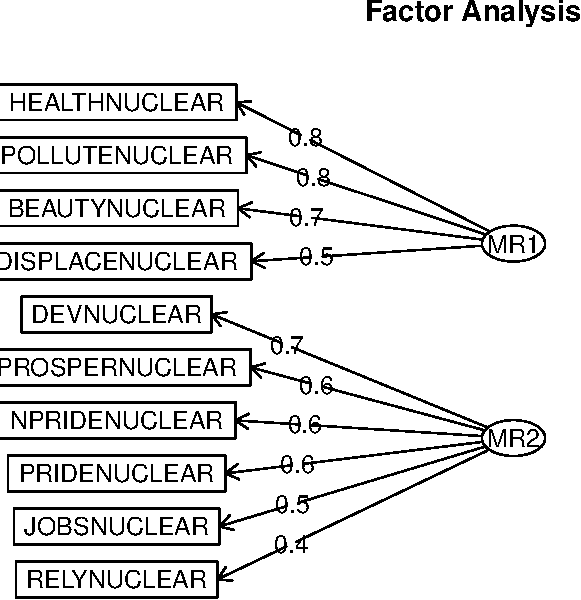
\includegraphics{module2PCAs_files/figure-latex/unnamed-chunk-10-1.pdf}
\newpage

\hypertarget{solar---fa-2-factor-solution}{%
\section{Solar - FA 2 factor
solution}\label{solar---fa-2-factor-solution}}

here I'll make the same chart with Coal as well - 2 factor solution and
explore the 4 factor solution. Talk to Terre about the Slovic study and
how they did it.

\begin{verbatim}
## 
## Reliability analysis   
##  raw_alpha std.alpha G6(smc) average_r S/N   ase mean  sd median_r
##       0.78      0.78    0.84      0.13 3.6 0.013  3.5 0.5     0.13
\end{verbatim}

\begin{verbatim}
## Factor Analysis using method =  minres
## Call: fa(r = secopolall, nfactors = 2, rotate = "varimax")
## Standardized loadings (pattern matrix) based upon correlation matrix
##               item   MR1   MR2    h2   u2 com
## DEVSOLAR        22  0.84       0.724 0.28 1.0
## PROSPERSOLAR    23  0.80       0.646 0.35 1.0
## PRIDESOLAR      20  0.80       0.656 0.34 1.1
## NPRIDESOLAR     21  0.78       0.616 0.38 1.0
## RELYSOLAR       24  0.60       0.361 0.64 1.0
## JOBSSOLAR       18  0.56       0.319 0.68 1.0
## ECONOMYLOCAL     8             0.124 0.88 1.2
## OWNERPVT        11             0.050 0.95 1.1
## POLLUTESOLAR    16        0.69 0.511 0.49 1.1
## HEALTHSOLAR     17        0.58 0.353 0.65 1.1
## BEAUTYSOLAR     19        0.55 0.304 0.70 1.0
## DISPLACESOLAR   15        0.54 0.290 0.71 1.0
## MECHANISATION    2       -0.52 0.300 0.70 1.2
## SYSTEMDEMO      25       -0.50 0.264 0.74 1.1
## ECONOMYGLOBAL    7        0.48 0.234 0.77 1.0
## OWNERPUB        13       -0.47 0.246 0.75 1.2
## ENVOVERDEV       9       -0.44 0.222 0.78 1.2
## OWNERREG        14       -0.44 0.191 0.81 1.0
## WEALTHLIM        1       -0.42 0.173 0.83 1.0
## INDUSTRYLARGE    5        0.41 0.180 0.82 1.1
## INDUSTRYSMALL    6             0.152 0.85 1.1
## DECISIONCEN      4             0.094 0.91 1.1
## DECISIONDECEN    3             0.063 0.94 1.0
## OWNERNOREG      12             0.071 0.93 1.4
## DEVOVERENV      10             0.061 0.94 1.3
## 
##                        MR1  MR2
## SS loadings           3.62 3.59
## Proportion Var        0.14 0.14
## Cumulative Var        0.14 0.29
## Proportion Explained  0.50 0.50
## Cumulative Proportion 0.50 1.00
## 
## Mean item complexity =  1.1
## Test of the hypothesis that 2 factors are sufficient.
## 
## The degrees of freedom for the null model are  300  and the objective function was  7.85 with Chi Square of  4522.16
## The degrees of freedom for the model are 251  and the objective function was  2.23 
## 
## The root mean square of the residuals (RMSR) is  0.08 
## The df corrected root mean square of the residuals is  0.08 
## 
## The harmonic number of observations is  586 with the empirical chi square  1982.05  with prob <  2.8e-266 
## The total number of observations was  586  with Likelihood Chi Square =  1279.58  with prob <  2.3e-137 
## 
## Tucker Lewis Index of factoring reliability =  0.708
## RMSEA index =  0.084  and the 90 % confidence intervals are  0.079 0.088
## BIC =  -320.12
## Fit based upon off diagonal values = 0.87
## Measures of factor score adequacy             
##                                                    MR1  MR2
## Correlation of (regression) scores with factors   0.95 0.91
## Multiple R square of scores with factors          0.90 0.83
## Minimum correlation of possible factor scores     0.81 0.67
\end{verbatim}

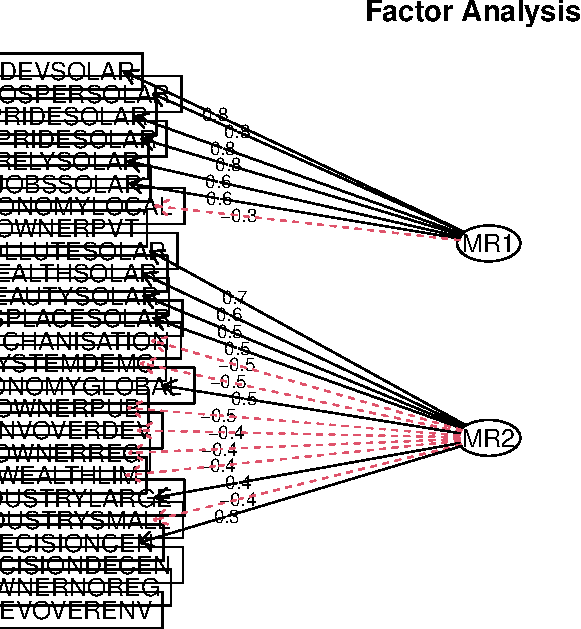
\includegraphics{module2PCAs_files/figure-latex/unnamed-chunk-11-1.pdf}

\newpage

\hypertarget{coal---fa-2-factor-solution}{%
\section{Coal - FA 2 factor
solution}\label{coal---fa-2-factor-solution}}

\begin{verbatim}
## 
## Reliability analysis   
##  raw_alpha std.alpha G6(smc) average_r S/N   ase mean   sd median_r
##        0.8       0.8    0.84      0.14 4.1 0.013  3.3 0.47     0.14
\end{verbatim}

\begin{verbatim}
## Factor Analysis using method =  minres
## Call: fa(r = cecopolall, nfactors = 2, rotate = "varimax")
## Standardized loadings (pattern matrix) based upon correlation matrix
##               item   MR1   MR2    h2   u2 com
## POLLUTECOAL     16  0.65       0.428 0.57 1.0
## BEAUTYCOAL      19  0.63       0.409 0.59 1.1
## MECHANISATION    2  0.58       0.361 0.64 1.1
## HEALTHCOAL      17  0.58       0.370 0.63 1.2
## DISPLACECOAL    15  0.54       0.295 0.71 1.0
## INDUSTRYSMALL    6  0.52       0.272 0.73 1.0
## OWNERREG        14  0.47       0.233 0.77 1.1
## SYSTEMDEMO      25  0.41       0.240 0.76 1.7
## JOBSCOAL        18  0.41       0.217 0.78 1.5
## DECISIONDECEN    3             0.128 0.87 1.0
## ECONOMYGLOBAL    7             0.183 0.82 2.0
## ENVOVERDEV       9             0.095 0.91 1.1
## WEALTHLIM        1             0.166 0.83 2.0
## OWNERPUB        13             0.101 0.90 1.5
## ECONOMYLOCAL     8             0.017 0.98 2.0
## PRIDECOAL       20        0.65 0.438 0.56 1.1
## NPRIDECOAL      21        0.59 0.374 0.63 1.2
## INDUSTRYLARGE    5       -0.44 0.246 0.75 1.5
## DEVCOAL         22        0.43 0.289 0.71 1.8
## PROSPERCOAL     23             0.229 0.77 1.9
## RELYCOAL        24             0.100 0.90 1.5
## DECISIONCEN      4             0.101 0.90 1.6
## OWNERNOREG      12             0.100 0.90 1.7
## OWNERPVT        11             0.060 0.94 1.7
## DEVOVERENV      10             0.022 0.98 1.2
## 
##                        MR1  MR2
## SS loadings           3.48 2.00
## Proportion Var        0.14 0.08
## Cumulative Var        0.14 0.22
## Proportion Explained  0.64 0.36
## Cumulative Proportion 0.64 1.00
## 
## Mean item complexity =  1.4
## Test of the hypothesis that 2 factors are sufficient.
## 
## The degrees of freedom for the null model are  300  and the objective function was  5.26 with Chi Square of  2554.39
## The degrees of freedom for the model are 251  and the objective function was  1.78 
## 
## The root mean square of the residuals (RMSR) is  0.07 
## The df corrected root mean square of the residuals is  0.07 
## 
## The harmonic number of observations is  496 with the empirical chi square  1261.39  with prob <  3.5e-134 
## The total number of observations was  496  with Likelihood Chi Square =  862.72  with prob <  4.2e-68 
## 
## Tucker Lewis Index of factoring reliability =  0.675
## RMSEA index =  0.07  and the 90 % confidence intervals are  0.065 0.075
## BIC =  -695.13
## Fit based upon off diagonal values = 0.87
## Measures of factor score adequacy             
##                                                    MR1  MR2
## Correlation of (regression) scores with factors   0.90 0.85
## Multiple R square of scores with factors          0.82 0.71
## Minimum correlation of possible factor scores     0.63 0.43
\end{verbatim}

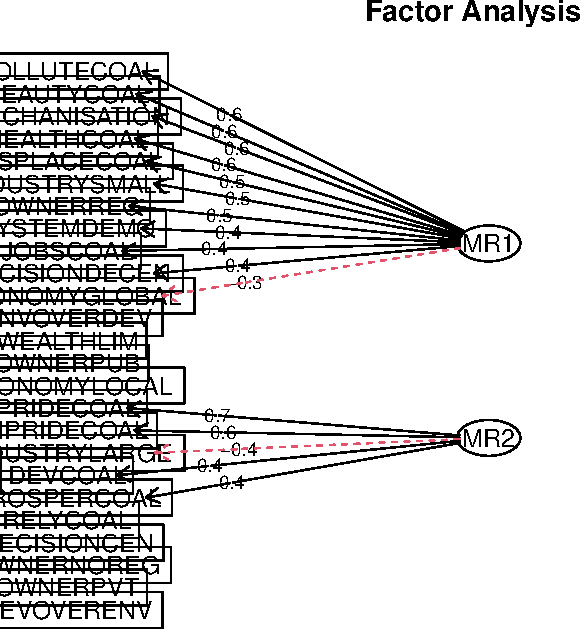
\includegraphics{module2PCAs_files/figure-latex/unnamed-chunk-12-1.pdf}

\newpage

\hypertarget{appendix1}{%
\section{Appendix1}\label{appendix1}}

\textbf{Kahan et al (2007) scale}

Individualism - Communitarinism

\begin{itemize}
\tightlist
\item
  \textbf{K\_IINTRFER} The government interferes far too much in our
  everyday lives.
\item
  \textbf{K\_IPRIVACY} The government should stop telling people how to
  live their lives.
\item
  \textbf{K\_IPROTECT} It's not the government's business to try to
  protect people from themselves.
\item
  \textbf{K\_SHARM} Sometimes the government needs to make laws that
  keep people from hurting themselves.
\item
  \textbf{K\_SLIMCHOI} The government should put limits on the choices
  individuals can make so they don't get in the way of what's good for
  society.
\item
  \textbf{K\_SPROTECT} The government should do more to advance
  society's goals, even if that means limiting the freedom and choices
  of individuals.
\end{itemize}

Hierarchy -Egalitarianism

\begin{itemize}
\tightlist
\item
  \textbf{K\_HEQUAL} We have gone too far in pushing equal rights in
  this country.
\item
  \textbf{K\_HREVDIS1} Nowadays it seems like there is just as much
  discrimination against upper castes as there is against Dalits.
\item
  \textbf{K\_EDISCRIM} Discrimination against minorities is still a very
  serious problem in our society.
\item
  \textbf{K\_ERADEQ1} We need to dramatically reduce inequalities
  between the rich and the poor.
\item
  \textbf{K\_EWEALTH} Our society would be better off if the
  distribution of wealth was more equal.
\item
  \textbf{K\_ERADEQ2} We need to dramatically reduce inequalities
  between men and women.
\end{itemize}

\newpage

\hypertarget{appendix2}{%
\section{Appendix2}\label{appendix2}}

\textbf{New Eco-pol values scale}

\begin{itemize}
\item
  \textbf{DISPLACENUCLEAR}Nuclear energy is leading to displacement of
  people from their land
\item
  \textbf{BEAUTYNUCLEAR} Nuclear energy spoils the natural beauty of the
  landscape
\item
  \textbf{POLLUTENUCLEAR} Nuclear energy increases pollution of
  air/water/land
\item
  \textbf{HEALTHNUCLEAR} Nuclear energy poses a great risk to the health
  of people living around it
\item
  \textbf{JOBSNUCLEAR} Nuclear energy will bring jobs to the local
  community
\item
  \textbf{PRIDENUCLEAR} I would be proud if my community used nuclear
  energy
\item
  \textbf{NPRIDENUCLEAR} Nuclear energy is a mark of pride for our
  nation
\item
  \textbf{DEVNUCLEAR} Nuclear energy pushes forward the country's
  development
\item
  \textbf{PROSPERNUCLEAR} Nuclear energy brings economic prosperity to
  the surrounding regions
\item
  \textbf{RELYNUCLEAR} I don't like the idea that I have to rely on the
  government for electricity from nuclear energy
\item
  \textbf{DECISIONDECEN} Local politicians shouldn't have to ask
  permission from the central government to implement policies
\item
  \textbf{DECISIONCEN} Laws and policies would be implemented more
  smoothly if more power lay with the central government.
\item
  \textbf{INDUSTRYLARGE} Large scale industries are required for the
  development of the country that will benefit everyone
\item
  \textbf{ECONOMYLOCAL} India would be better off if foreign companies
  didn't come to here
\item
  \textbf{DEVOVERENV} Economic growth and creating jobs should be
  prioritized over environmental protection
\item
  \textbf{INDUSTRYSMALL} Large corporations are destroying the local
  industries in India and benefiting only a handful of people.
\item
  \textbf{WEALTHLIM} A limit should be put to how much wealth a person
  can amass
\item
  \textbf{ECONOMYGLOBAL} Foreign companies have led to a range of
  benefits for the Indian people and society
\item
  \textbf{OWNERPVT} All businesses and industries should be owned
  privately
\item
  \textbf{OWNERPUB} The government should own most large businesses and
  industries
\item
  \textbf{ENVOVERDEV} Polluting industries that spoil the environment
  should be shut down even if it costs people their jobs
\item
  \textbf{OWNERREG} Regardless of ownership, the government should pass
  strong regulations and implement them
\item
  \textbf{MECHANISATION} Rapid mechanization of work is taking away jobs
  from workers in this country
\item
  \textbf{OWNERNOREG} There is too much red-tape and the government
  should not interfere with businesses and industries
\end{itemize}

\end{document}
